% Niveau :      PCSI *
% Discipline :  Géné
% Mots clés :   Diagrammes E-pH

\begin{exercise}{Titrage et diagramme $E$-pH}{2}{PCSI}
{Chimie générale, Réactions acidobasiques, Oxydoréduction, Diagrammes E-pH}{bermu}




\begin{questions}
\questioncours Lecture et construction de diagrammes $E$-pH.
\vspace{-1em}\begin{EnvUplevel}
Dans la figure \ref{fig:EpHS} en annexe est tracé le diagramme simplifié du soufre pour les espèces $\mathrm{S_{(s)}}$, $\mathrm{{HSO_4^-}_{(aq)}}$, $\mathrm{{SO_4^{2-}}_{(aq)}}$, $\mathrm{ {H_2S}_{(g)}}$, $\mathrm{{HS^-}_{(aq)}}$ et $\mathrm{{S^{2-}}_{(aq)}}$. \\[1ex]
\textsl{On tracera les diagrammes avec des couleurs différentes sur la figure en annexe. \\
Il ne sera exigé de calculer que les pentes de chaque frontière (tracé rapide).}
\end{EnvUplevel}
\begin{parts}
    \part En justifiant, ajouter au diagramme les domaines de prédominance / d'existence de ces espèces.
    \part Quelle est l'allure des frontières correspondant à des réactions acido-basiques ? \\
    Donner le p$K_a$ du couple $\mathrm{{HS^-}_{(aq)} / {S^{2-}}_{(aq)}}$.
    \part Quel est le potentiel standard du couple $\mathrm{{HSO_4^-}_{(aq)} / S_{(s)}}$ ?
    \part Tracer le diagramme $E$-pH de l'eau en donnant les équations des différentes frontières. \\
    \`A quoi correspondent ces trois domaines d'un point de vue chimique (mis à part les domaines de prédominance de chaque espèce) ?
    \part \`A l'aide des données, tracer le diagramme $E$-pH de l'iode.
\end{parts}

\begin{EnvUplevel}
On se propose d'étudier le protocole suivant :
\begin{enumerate}%[label={\bfseries{\itshape\alph*}\,)}]
    \item dans un bécher, introduire 20 mL d'une solution de $I_2$ à 0,1 M dans du KI saturé ;
    \item ajouter 20 mL d'une solution de soude à 2M ;
    \item introduire 20 mL d'une solution de sulfure de disodium de concentration $c \simeq 10^{-2}$ M inconnue ;
    \item chauffer avec agitation pendant 10 minutes ;
    \item après refroidissement, acidifier avec de l'acide sulfurique ;
    \item titrer avec une solution de Na$_2$S$_2$O$_3$ à 0,1 M.
\end{enumerate}

Après avoir effectué ce protocole, on trouve un volume à l'équivalence de $V_\text{éq} = 22,4$ mL.
\end{EnvUplevel}

    \question Interpréter le mode opératoire à l'aide de la figure \ref{fig:EpHS} en annexe et indiquer les réactions chimiques ayant lieu entre les différentes étapes.
    
    \question En déduire la concentration de la solution de Na$_2$S.

\end{questions}

\paragraph{Données : } potentiels standards $E^\circ$ dans les CNTP
\begin{center}\begin{tabularx}{.7\linewidth}{rCCC}
    \hline
    & $\mathrm{{I_3^-}_{(aq)} \,/\, {I^-}_{(aq)}}$
    & $\mathrm{{IO_3^-}_{(aq)} \,/\, {I_3^-}_{(aq)}}$
    & $\mathrm{{O_2}_{(g)} \,/\, {H_2O}_{(\ell)}}$ \\
    $E^\circ$ (V) & 0,53 & 1,18 & 1,23 \\
    $E^\circ / \varepsilon^\circ$ & 9,0 & 20 & 21 \\ \hline\hline 
\end{tabularx}
\end{center}

On note $\varepsilon^\circ = \dfrac{RT}{\scr{F}} \ln10 = 59$ mV.


\end{exercise}

\begin{nopagebreak}
    \exerciselabelformat{Annexe Exercice \arabic{exercise} \quad --- \quad} \textsl{\`A rendre avec la copie.}
    
    \begin{figure}[H]
        \centering
        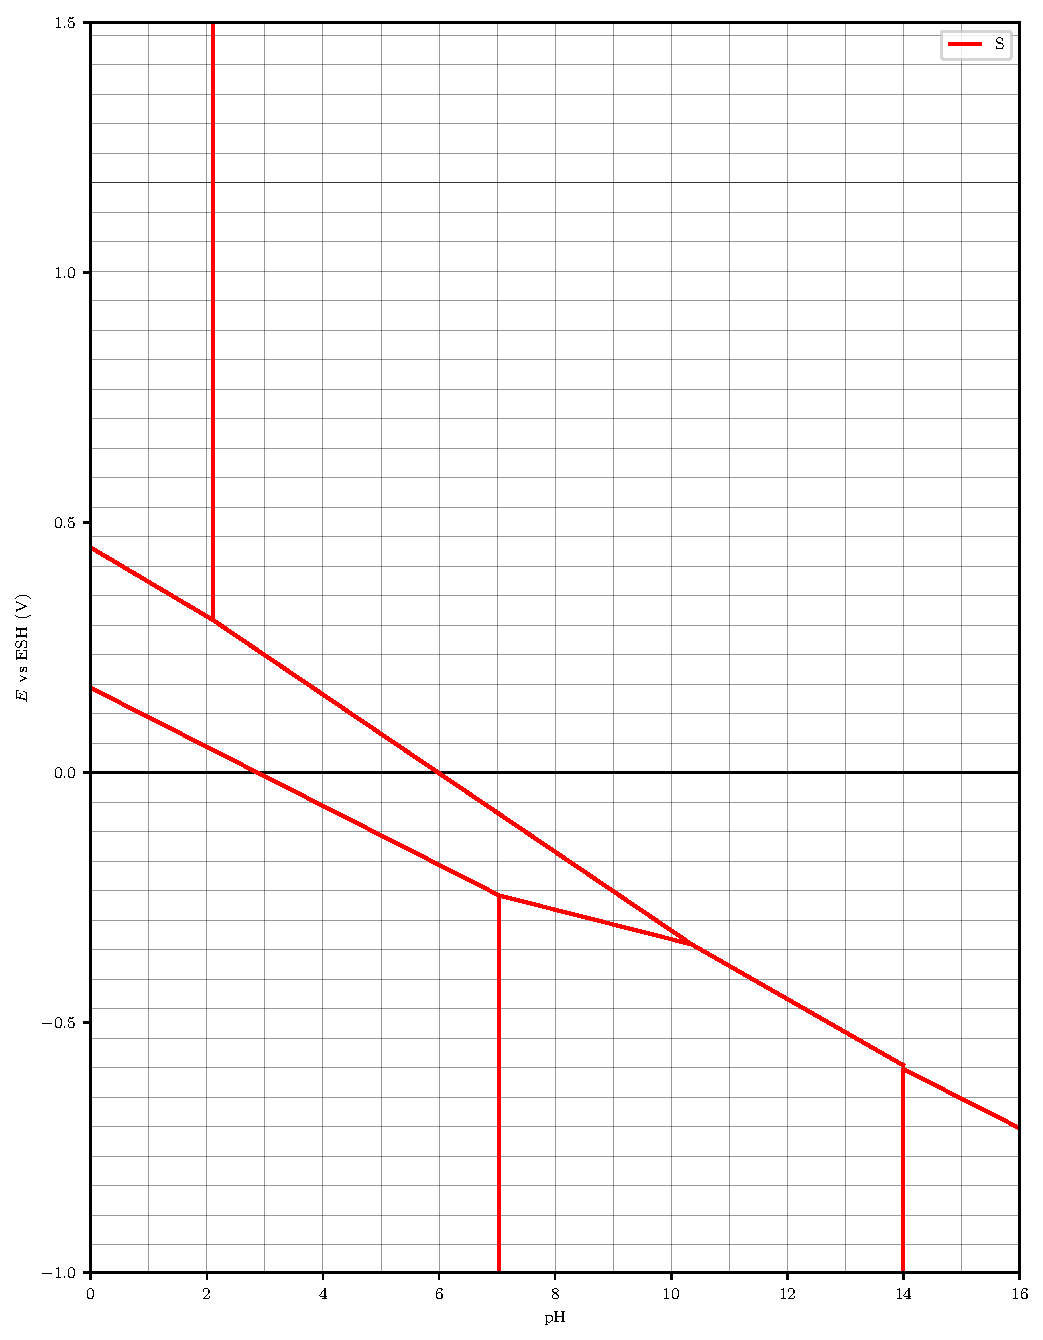
\includegraphics[width = \linewidth]{chimiePC/gene/E-pH-S.pdf}
        \caption{Diagramme $E$-pH simplifié du soufre avec une concentration de tracé de $0,1$ M. \protect\linebreak
        Le quadrillage est de $\varepsilon^\circ = 59$ mV par 1 unité de pH.}
        \label{fig:EpHS}
    \end{figure}
    
    \paragraph{Convention de tracé :}
\begin{itemize}
    \item les espèces en solution ont pour activité $c_\text{tr}/c^\circ = 10^{-1}$,
    \item les espèces gazeuses ont pour activité $p_\text{tr}/p^\circ = 10^{-2}$,
    \item les espèces solides ont pour activité $1$.
\end{itemize}

\end{nopagebreak}

\begin{solution}
\begin{questions}
\questioncours cf. le diagramme complété

\begin{parts}
    \part Les espèces du soufre ont les D.O. suivant : S$_{(s)}$ D.O. = 0 ; H$_2$S, HS$^-$, S$^{2-}$ : -II ; HSO$_4^-$ , SO$_4^{2-}$ : +VI.
    On remplit du bas vers le haut par D.O. croissant puis pour les espèces au même D.O. on place les espèces acide à gauche et basique à droite.
    
    \part Frontière verticale car pas d'échange d'électrons
   On lit sur le diagramme le pK$_a$=14.
    \part Le couple $\mathrm{{HSO_4^-}_{(aq)} / S_{(s)}}$ de demi-équation redox : HSO$_4^-$ + 7H$^+$ + 6e$^-$ = S$_{(s)}$ + 4H$_2$O.
    
    La formule de Nernst donne donc  $E = E^\circ(HSO_4^-/S_{(s)}) + \frac{0,06}{6}log([H^+]^7 \times [HSO_4^-])$.
    
    On lit sur le diagramme l'ordonnée à l'origine de la frontière entre ces deux espèces : E(pH=0) = 0,44V = $E^\circ(HSO_4^-/S_{(s)}) + 0,01\times log(10^{-1})$ d'ou $E^\circ(HSO_4^-/S_{(s)})$ = 0,45 V. 
    \part cf. cours
    Le domaine de l'eau liquide correspond au domaine de stabilité thermodynamique des espèces dans l'eau. 
    
    \part \`A l'aide des données, tracer le diagramme $E$-pH de l'iode.
\end{parts}

    \question 
    \begin{enumerate}%[label={\bfseries{\itshape\alph*}\,)}]
    \item  I$_2$ + I$^- \rightleftarrows$ I$_3^-$ 
    
    Comme KI est en excès cette réaction est quantitative on forme donc 2mmol de I$_3^-$
    
    \item On remarque qu'en milieu basique I$_3^-$ n'est pas stable et dismute en I$^-$ et IO$_3^-$ selon l'équation : 
    3I$_3^-$ + 6OH$^- \rightleftarrows$ 8I$^-$ + IO$_3^-$ + 3H$_2$O 
    
    A pH très basique, cette réaction est totale. On forme donc $\frac{2}{3}$ mmol de IO$_3^-$ et $\frac{16}{3}$ mmol de I$^-$. 
    
    \item On voit sur le diagramme que S$^{2-}$ et IO$_3^-$ ont des domaines disjoints et donc vont réagir ensemble selon l'équation : 
    
    4IO$_3^-$ + 3S$^{2-} \rightleftarrows$ 4I$^-$ + 3SO$_4^{2-}$ 
    
    Le réactif limitant est S$^{2-}$ (n(S$^{2-}) \approx$ 0,2 mmol) et donc après cette étape il reste $n = \frac{2}{3}-4\times\frac{n(S^{2-})}{3}$ $\approx$ 0,4 mmol de IO$_3^-$
    
    \item On acidifie donc la réaction de dismutation a lieu dans l'autre sens (mediamutation) (il y a toujours du KI en excès dans la solution) 
    
    8I$^-$ + IO$_3^-$ + 6H$^+$ $\rightleftarrows$ 3I$_3^-$ + 3H$_2$O
    
    IO$_3^-$ est le réactif limitant car I$^-$ est en excès, on forme donc 2-4$\times$n(S$^{2-}$) mmol de I$_3^-$.
    
    \item On dose le I$_3^-$ formé avec le thiosulfate de sodium selon l'équation :
    
    I$_3^-$ + 2S$_2$O$_3^{2-} \rightleftarrows$ 3I$^-$ + S$_4$O$_6^{2-}$ 

    \end{enumerate}
    
    \question Vu l'équation précédente, on a à l'équivalence $n_\mathrm{I_3^-} = 2-4\times [\text{S}^{2-}]\times 20 = \frac{1}{2} \mathrm{[Na_2S_2O_3]} V_\text{eq}$, d'où $c = 0,011$ M.

\end{questions}

    \begin{figure}[H]
        \centering
        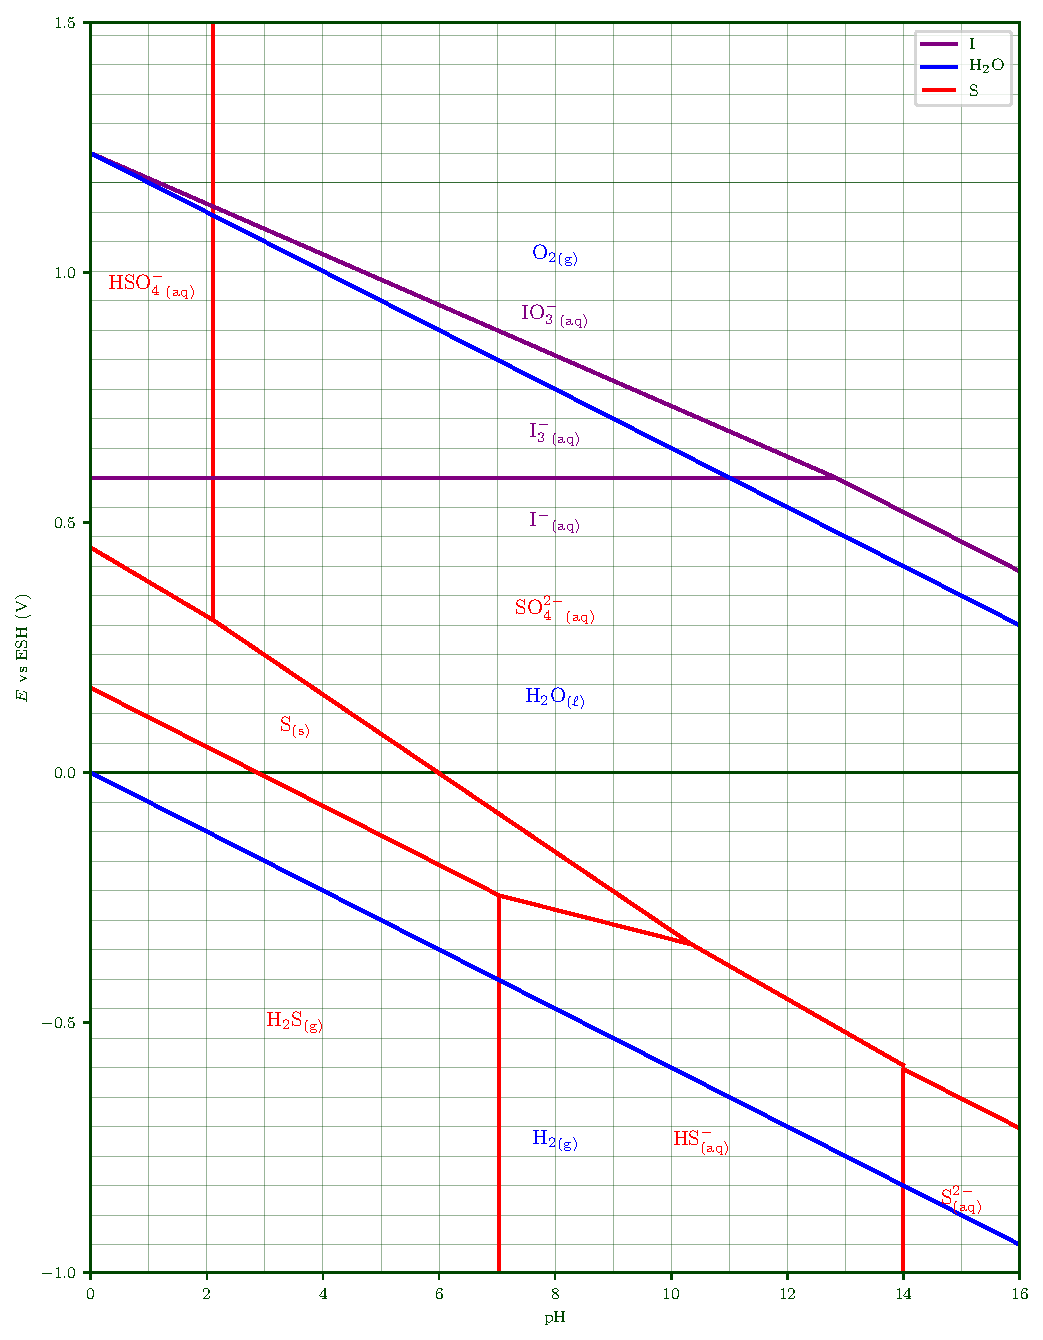
\includegraphics[width = \linewidth]{chimiePC/gene/E-pH-S-sol.pdf}
        \caption{Diagrammes $E$-pH superposés du soufre, de l'iode et de l'eau. \protect\linebreak
        Le quadrillage est de $\varepsilon^\circ = 59$ mV par 1 unité de pH.}
        \label{fig:EpHS-sol}
    \end{figure}
    
\end{solution}